\section{Differentials as covectors and their transformation rules}

Let's start this chapter by reminind ourselves what differentials are and covectors are.
We know that differentials in Integrals, like $dx$ are small changes in the variable of integration, in this case it's a small 
change in the variable x.\\

Covectors instead, are these functionals acting on vectors, and outputting scalars, which can be visualized as stacks of lines that
indeed eat a vector and produce a scalar. The scalar can be tought as the number of times the vector pierces the stack of lines.\\

\textbf{So like, how can these two concepts be linked together, and actually how the hell are they the same thing?}\\

The key of understanding this, is the re-interpretation of the $d$ symbol of the differentials.
The old way of thinking about it, is that this symbol takes the variable and gives a small change of this variable.\\
The new interpretation is that $d$ is an operator that takes a scalar field $f$ and outputs a $df$ covector field.
A scalar field is a field where a scalar $f$ is defined at every point in space, a covector field $df$ is a field 
where a covector is defined at every point in space.\\

So how does this $d$ operator work? A couple of pictures are worth a thousand words here:

\begin{center}
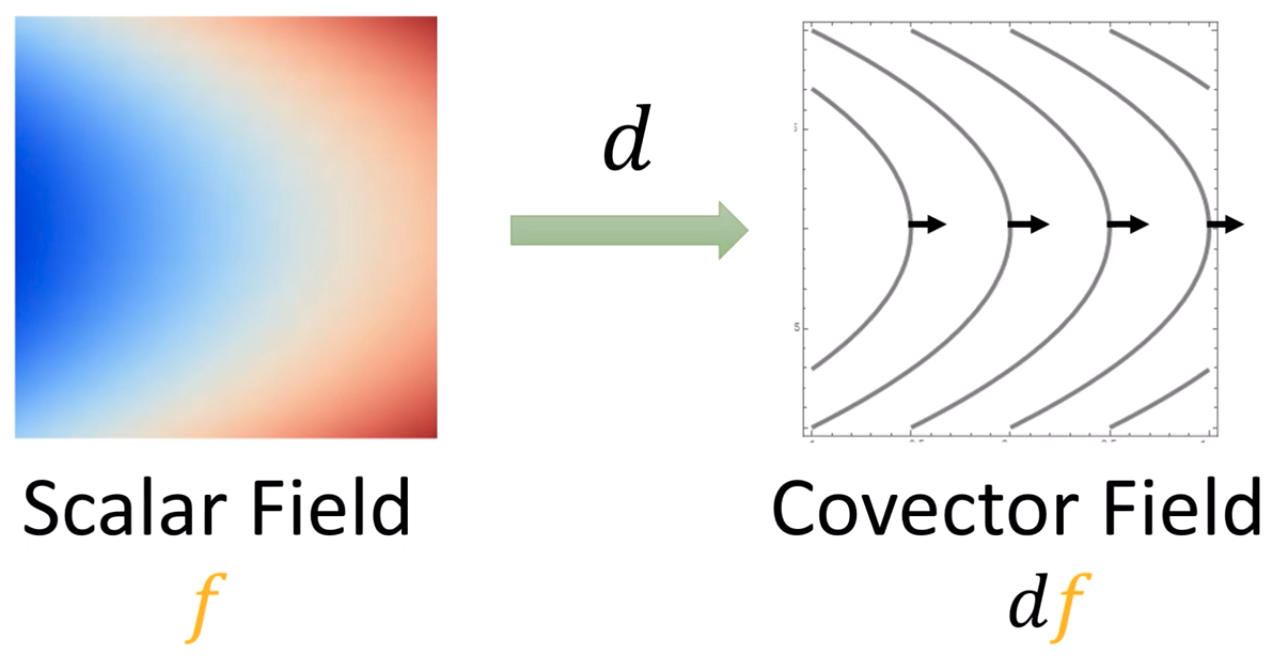
\includegraphics[scale=0.2]{figures/scalar-field-covector-field-01.png}
\end{center}

\begin{center}
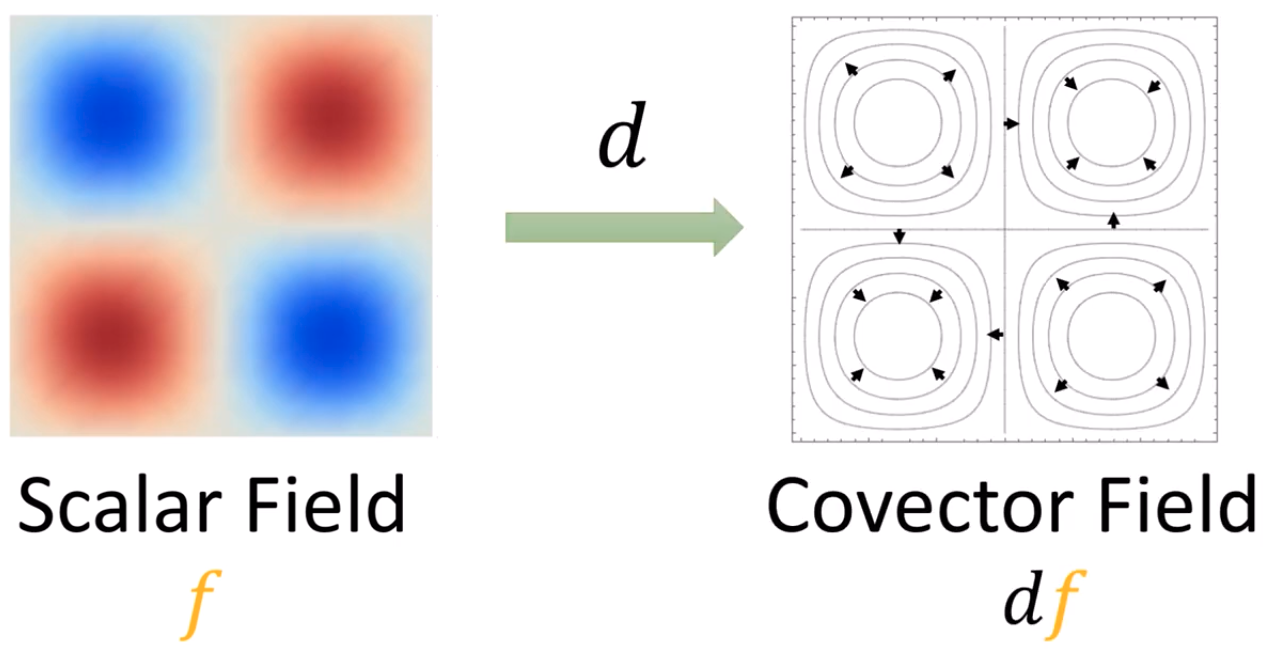
\includegraphics[scale=0.2]{figures/scalar-field-covector-field-02.png}
\end{center}

So like, the operator $d$ takes a function and outputs the function's level sets.
Sometimes, they're called 0-forms (functions) and 1-forms (level sets).\\

Let's give another example, showing the covector fields of the cartesian coordinates $dx$ and $dy$:

\begin{center}
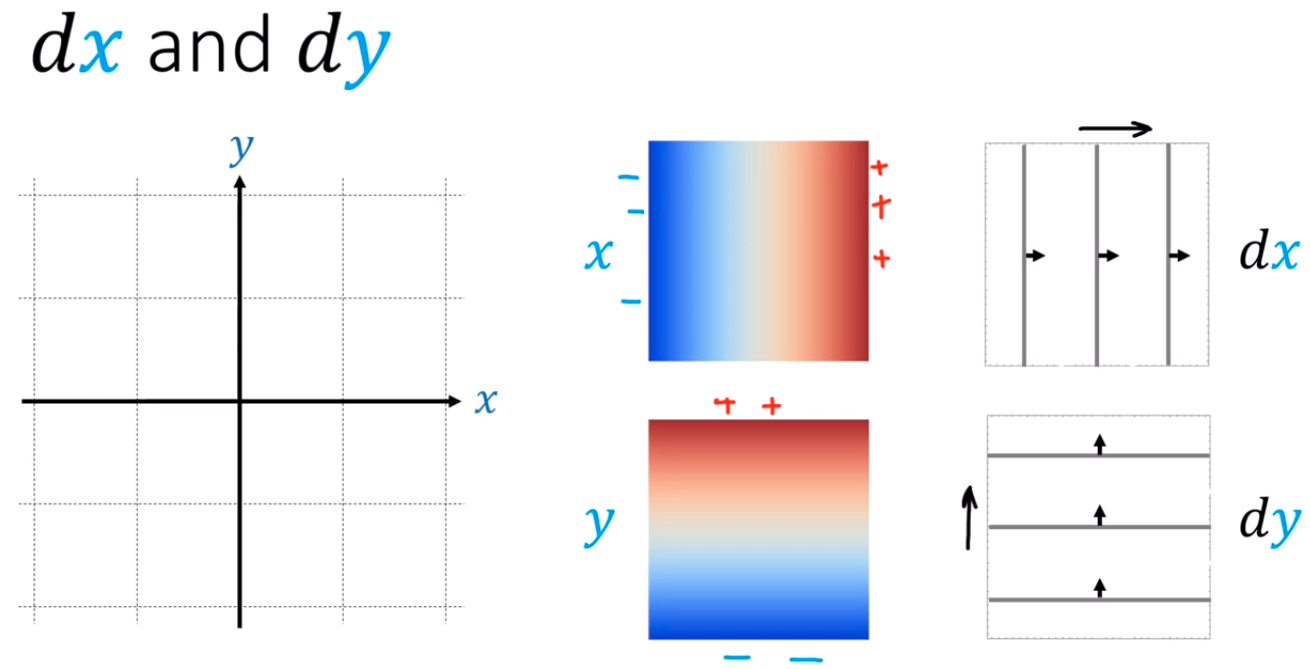
\includegraphics[scale=0.3]{figures/cartesian-covector-field.png}
\end{center}

Now, if this operator is really a covector field, we know that covectors eat vectors to output scalars, right?
How does this work considering what we've seen so far?

\begin{center}
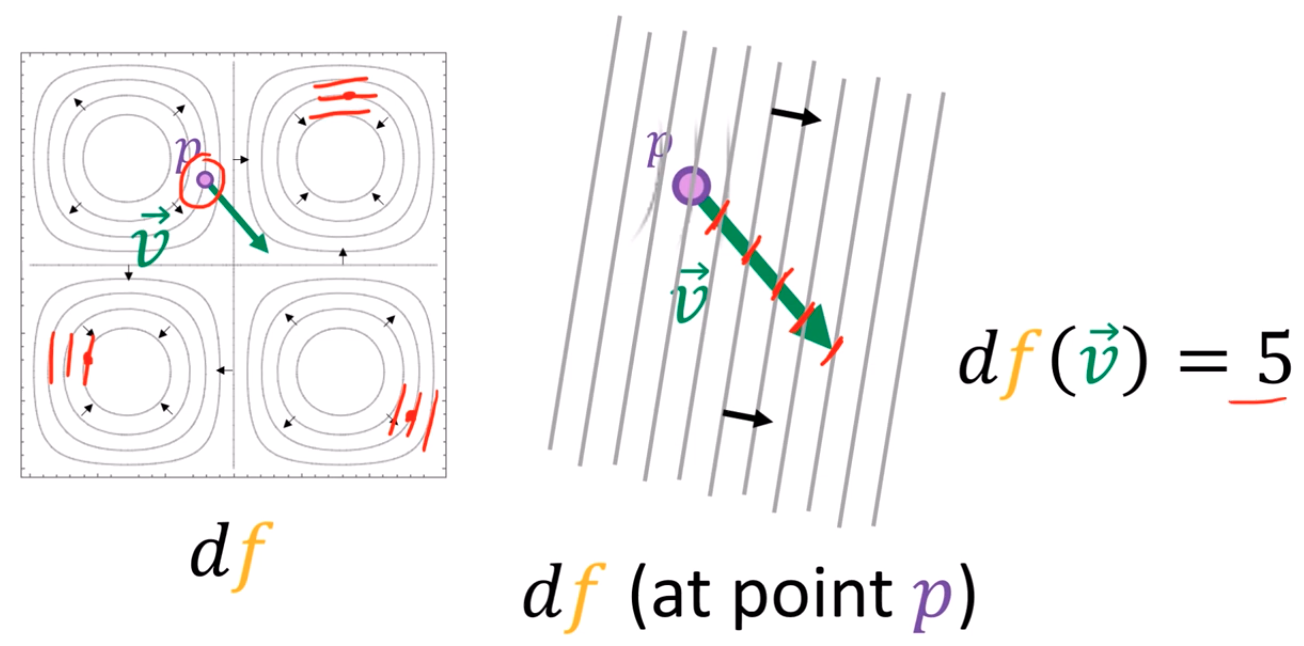
\includegraphics[scale=0.3]{figures/covector-field-on-vector.png}
\end{center}

And it's also quite straight forward to show that covector fields are linear.
But whet's the geometrical meaning of $d\begingroup\color{orange}f\endgroup(\begingroup\color{teal}\vec{v}\endgroup)$

\begin{center}
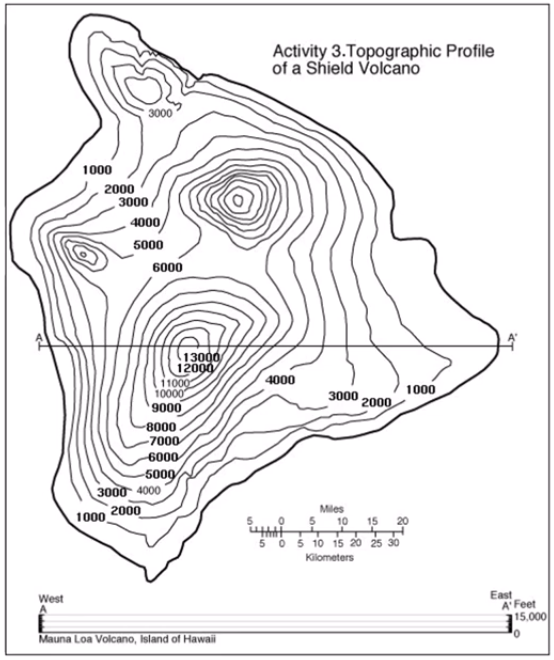
\includegraphics[scale=0.4]{figures/level-set-map.png}
\end{center}

We can think of these level sets of a map as a covector field.\\
When acting on a vector, $d\begingroup\color{orange}f\endgroup(\begingroup\color{teal}\vec{v}\endgroup)$ is proportional to the steepness of $\color{orange}f$ in the 
direction of $\color{teal}\vec{v}$ and also proportional to the length of $\color{teal}\vec{v}$.\\

So: \textbf{$d\begingroup\color{orange}f\endgroup(\begingroup\color{teal}\vec{v}\endgroup)$ tells us the rate of change of $\color{orange}f$
when moving at velocity $\color{teal}\vec{v}$}\\

But then, this reminds us of the definition of directional derivative, isn't it?
At the end of the day, $d\begingroup\color{orange}f\endgroup(\begingroup\color{teal}\vec{v}\endgroup)$ is the \textbf{directional derivative} of the function in the vector direction.

\begin{equation}
    d\begingroup\color{orange}f\endgroup(\begingroup\color{teal}\vec{v}\endgroup) = D_{\begingroup\color{teal}\vec{v}\endgroup}\begingroup\color{orange}f\endgroup
    = \frac{\partial \begingroup\color{orange}f\endgroup}{\partial \begingroup\color{teal}\vec{v}\endgroup}
\end{equation}

\subsection{Differential forms components and their transformation}
Just as we can write vectors as linear combinations of special basis vectors, scaled by some components, we can 
break covector fields, or differential forms, as linear combination of some special differential forms basis scaled by their components.\\

\begin{equation}
    d\begingroup\color{orange}f\endgroup = \begingroup\color{red} A \endgroup d\begingroup\color{cyan}x\endgroup + \begingroup\color{red} B \endgroup d\begingroup\color{cyan}y\endgroup
\end{equation}

Let's start by checking how differential forms act on our special basis vectors $\frac{\partial}{\partial x}, \frac{\partial}{\partial y}$:

\begin{equation}
    d\begingroup\color{orange}f\endgroup (\begingroup\color{blue}\vec{e_x}\endgroup) = 
    d\begingroup\color{orange}f\endgroup \left(\frac{\partial}{\partial \begingroup\color{cyan}x\endgroup}\right) = \frac{\partial \begingroup\color{orange}f\endgroup}{\partial \begingroup\color{cyan}x\endgroup}
\end{equation}

That's the directional derivative of $f$ in the $x$ direction.\\ 
Same for the other direction:

\begin{equation}
    d\begingroup\color{orange}f\endgroup (\begingroup\color{blue}\vec{e_y}\endgroup) = 
    d\begingroup\color{orange}f\endgroup \left(\frac{\partial}{\partial \begingroup\color{cyan}y\endgroup}\right) = \frac{\partial \begingroup\color{orange}f\endgroup}{\partial \begingroup\color{cyan}y\endgroup}
\end{equation}

Now we can look at the simple scalar field $\color{cyan}x$, and the scalar value at a point is just the value of $x$ at that point, positives on the right, negative on the left.\\
The corresponding covector field is $d\color{cyan}x$, represented by vertical level sets directed to the right.\\
So:

\begin{align*}
    d\begingroup\color{cyan}x\endgroup (\begingroup\color{blue}\vec{e_x}\endgroup) &= d\begingroup\color{cyan}x\endgroup \left(\frac{\partial}{\partial \begingroup\color{cyan}x\endgroup}\right)\\
    &= \frac{\partial \begingroup\color{cyan}x\endgroup}{\partial \begingroup\color{cyan}x\endgroup} = 1\\
    d\begingroup\color{cyan}x\endgroup (\begingroup\color{blue}\vec{e_y}\endgroup) &= d\begingroup\color{cyan}x\endgroup \left(\frac{\partial}{\partial \begingroup\color{cyan}y\endgroup}\right)\\
    &= \frac{\partial \begingroup\color{cyan}x\endgroup}{\partial \begingroup\color{cyan}y\endgroup} = 0
\end{align*}

Same process can be applied to the scalar field $\color{cyan}y$, obtaining in summary:

\begin{align*}
    d\begingroup\color{cyan}x\endgroup \left(\frac{\partial}{\partial \begingroup\color{cyan}x\endgroup}\right) = \frac{\partial \begingroup\color{cyan}x\endgroup}{\partial \begingroup\color{cyan}x\endgroup} = 1 && 
    d\begingroup\color{cyan}x\endgroup \left(\frac{\partial}{\partial \begingroup\color{cyan}y\endgroup}\right) = \frac{\partial \begingroup\color{cyan}x\endgroup}{\partial \begingroup\color{cyan}y\endgroup} = 0\\
    d\begingroup\color{cyan}y\endgroup \left(\frac{\partial}{\partial \begingroup\color{cyan}x\endgroup}\right) = \frac{\partial \begingroup\color{cyan}y\endgroup}{\partial \begingroup\color{cyan}x\endgroup} = 0 && 
    d\begingroup\color{cyan}y\endgroup \left(\frac{\partial}{\partial \begingroup\color{cyan}y\endgroup}\right) = \frac{\partial \begingroup\color{cyan}y\endgroup}{\partial \begingroup\color{cyan}y\endgroup} = 1
\end{align*}

Which can be re-written, considering $\begingroup\color{cyan}c^1\endgroup = \begingroup\color{blue}x\endgroup, \begingroup\color{cyan}c^2\endgroup = \begingroup\color{blue}y\endgroup$:

\begin{equation}
    d\begingroup\color{cyan}c^i\endgroup \left(\frac{\partial}{\partial \begingroup\color{cyan}c^j\endgroup}\right) = \frac{\partial \begingroup\color{cyan}c^i\endgroup}{\partial \begingroup\color{cyan}c^j\endgroup} = \delta^i_j
\end{equation}

As when we discussed the special dual basis (co)vectors in the "Tensor for Beginners" notes, these special differential forms $d\color{cyan}x$, $d\color{cyan}y$ are the
dual basis for differential forms.\\
To find the coefficients, let's just consider a generic function $\begingroup\color{orange}f\endgroup (\begingroup\color{cyan}x, y\endgroup)$ and a curve parametrized by the parameter $\color{brown}\lambda$.\\
The tangent vectors along the curve are given by $\frac{\partial}{\partial \color{brown}\lambda}$.\\
Let's consider the rate of change of this function as we travel along the curve, which is given by the derivative $\frac{d \begingroup\color{orange}f\endgroup}{d \begingroup\color{brown}\lambda\endgroup}$\\

Now remember this, the covector field $df$, acting on the vector $d/d\lambda$ is equal to $df/d\lambda$ so we can re-write:

\begin{align*}
    \frac{d\begingroup\color{orange}f\endgroup}{d \begingroup\color{brown}\lambda\endgroup} &=
    \frac{\partial \begingroup\color{orange}f\endgroup}{\partial \begingroup\color{cyan}x\endgroup} \frac{d \begingroup\color{cyan}x\endgroup}{d \begingroup\color{brown}\lambda\endgroup} +
    \frac{\partial \begingroup\color{orange}f\endgroup}{\partial \begingroup\color{cyan}y\endgroup} \frac{d \begingroup\color{cyan}y\endgroup}{d \begingroup\color{brown}\lambda\endgroup}\\
    d\begingroup\color{orange}f\endgroup \left(\frac{d}{d \begingroup\color{brown}\lambda\endgroup}\right) &=
    \frac{\partial \begingroup\color{orange}f\endgroup}{\partial \begingroup\color{cyan}x\endgroup} d\begingroup\color{cyan}x\endgroup \left(\frac{d }{d \begingroup\color{brown}\lambda\endgroup}\right) +
    \frac{\partial \begingroup\color{orange}f\endgroup}{\partial \begingroup\color{cyan}y\endgroup} d\begingroup\color{cyan}y\endgroup \left(\frac{d }{d \begingroup\color{brown}\lambda\endgroup}\right)\\
    d\begingroup\color{orange}f\endgroup \left(\frac{d}{d \begingroup\color{brown}\lambda\endgroup}\right) &=
    \left(\frac{\partial \begingroup\color{orange}f\endgroup}{\partial \begingroup\color{cyan}x\endgroup} d\begingroup\color{cyan}x\endgroup + \frac{\partial \begingroup\color{orange}f\endgroup}{\partial \begingroup\color{cyan}y\endgroup} d\begingroup\color{cyan}y\endgroup\right)
    \left(\frac{d}{d \begingroup\color{brown}\lambda\endgroup}\right)
\end{align*}

So from the last equation, we can deduce that these two quantities are the same vector field:

\begin{equation}
    d\begingroup\color{orange}f\endgroup = \frac{\partial \begingroup\color{orange}f\endgroup}{\partial \begingroup\color{cyan}x\endgroup} d\begingroup\color{cyan}x\endgroup + \frac{\partial \begingroup\color{orange}f\endgroup}{\partial \begingroup\color{cyan}y\endgroup} d\begingroup\color{cyan}y\endgroup
\end{equation}

And this is indeed what we were looking for, writing the covector field as linear combination of $d\color{cyan}x$, $d\color{cyan}y$, so $d\color{cyan}x$, $d\color{cyan}y$ form a basis for 
the set of covector fields. They're the dual basis for differential forms.\\

Let's see a more concrete example to understand this better.
Consider this scalar field, we can write down the covector field in terms of the basis vectors in this way:

\begin{center}
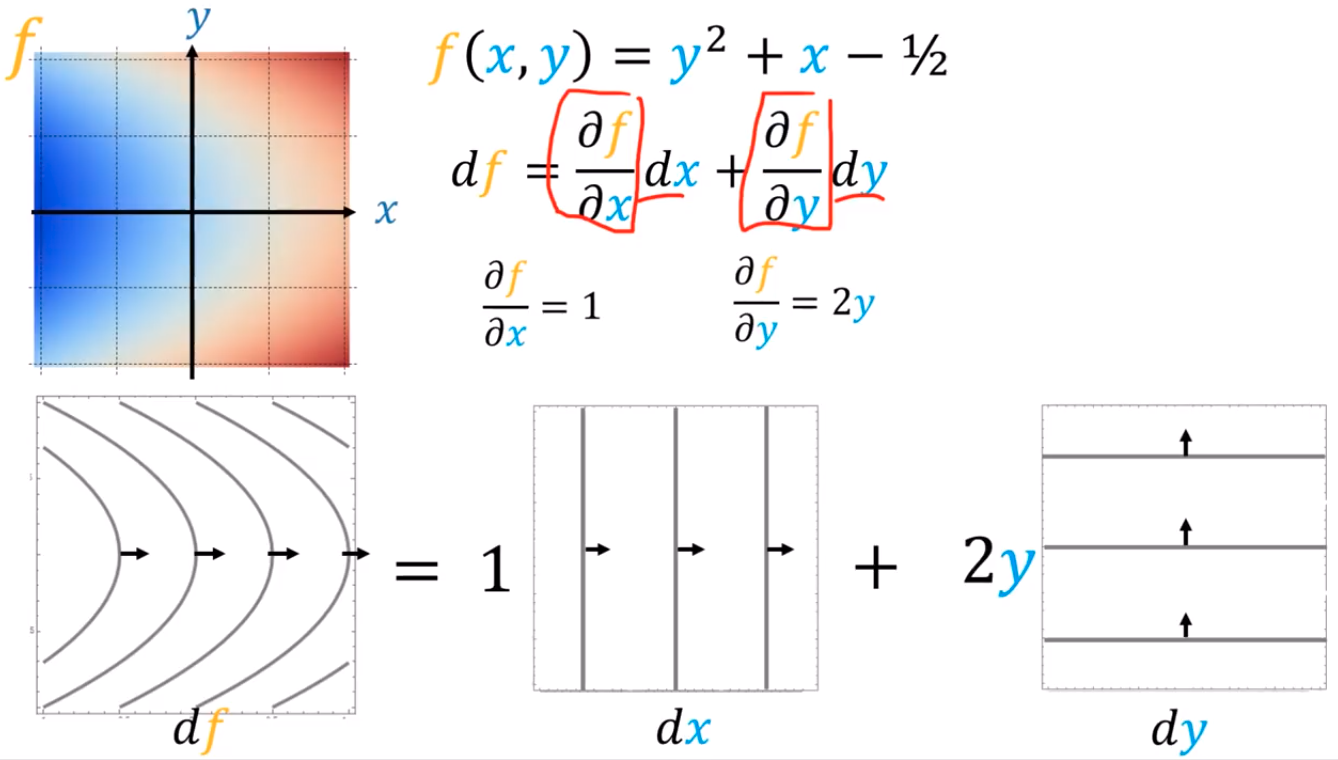
\includegraphics[scale=0.3]{figures/covector-components-ex-01.png}
\end{center}

The same can be done in other coordinate systems, like polar ones:

\begin{center}
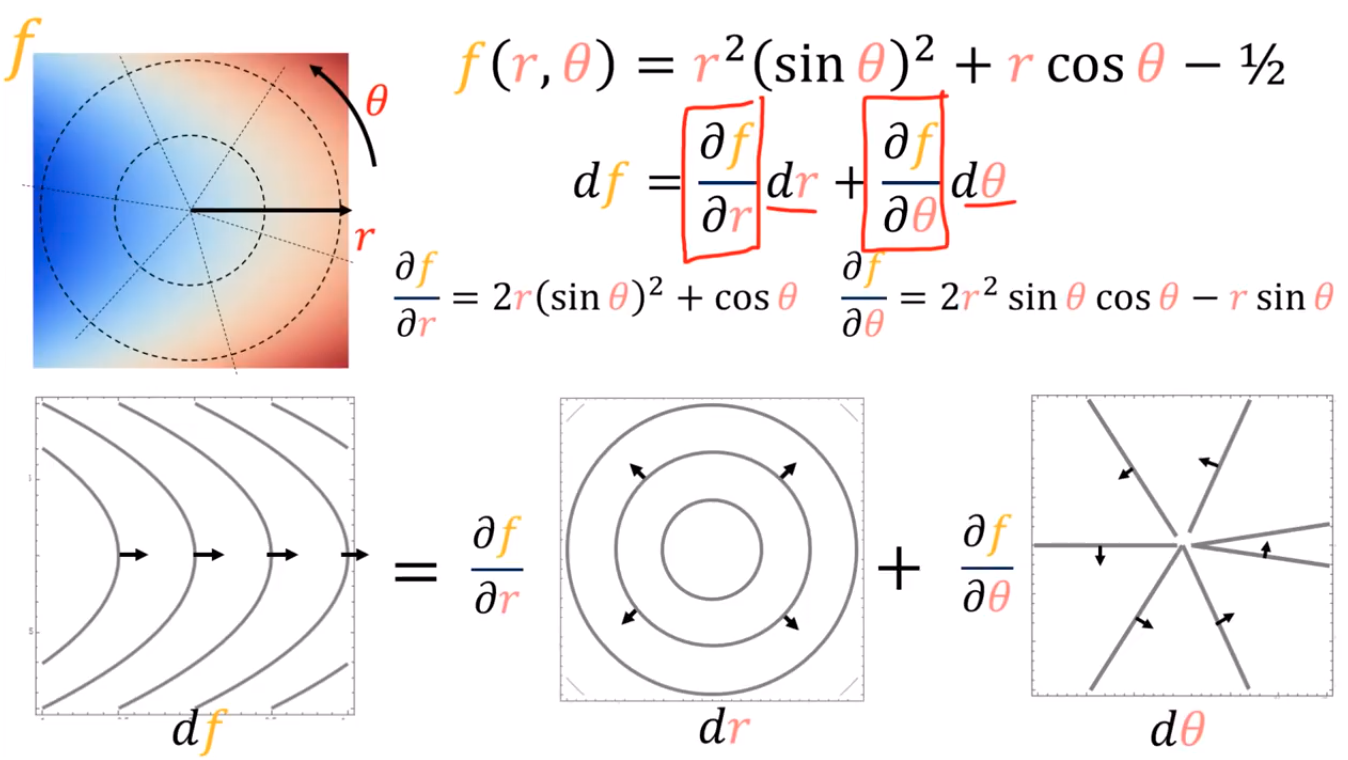
\includegraphics[scale=0.3]{figures/covector-components-polar-ex-01.png}
\end{center}

Now, how would both the covector basis field and the covector field components transform?
Well we just showed that any covector field can be written as linear combination of basis covector field $d\begingroup\color{cyan}x\endgroup$ and $d\begingroup\color{cyan}y\endgroup$.\\

But since this is valid for any covector field, we can expand our new polar covector field basis:

\begin{align*}
    d\begingroup\color{magenta}r\endgroup = \frac{\partial \begingroup\color{magenta}r\endgroup}{\partial \begingroup\color{cyan}x\endgroup} d\begingroup\color{cyan}x\endgroup + \frac{\partial \begingroup\color{magenta}r\endgroup}{\partial \begingroup\color{cyan}y\endgroup} d\begingroup\color{cyan}y\endgroup\\
    d\begingroup\color{magenta}\theta\endgroup = \frac{\partial \begingroup\color{magenta}\theta\endgroup}{\partial \begingroup\color{cyan}x\endgroup} d\begingroup\color{cyan}x\endgroup + \frac{\partial \begingroup\color{magenta}\theta\endgroup}{\partial \begingroup\color{cyan}y\endgroup} d\begingroup\color{cyan}y\endgroup\\
\end{align*}

If you recall, those coefficients are just the entries of the Inverse Jacobian Matrix $B$ or $J^{-1}$.
What this means is that, covector basis field transform contravariantly.\\
In Einstein notation, and then in matrix notation, we can write:

\begin{align*}
    d\begingroup\color{magenta}p^i\endgroup &= \frac{\partial \begingroup\color{magenta}p^i\endgroup}{\partial \begingroup\color{cyan}c^j\endgroup} d\begingroup\color{cyan}c^j\endgroup\\
    \begin{bmatrix}
        d\begingroup\color{magenta}r\endgroup\\
        d\begingroup\color{magenta}\theta\endgroup
    \end{bmatrix} &= 
    \begin{bmatrix}
        \frac{\partial \begingroup\color{magenta}r\endgroup}{\partial \begingroup\color{cyan}x\endgroup} & \frac{\partial \begingroup\color{magenta}r\endgroup}{\partial \begingroup\color{cyan}y\endgroup}\\
        \frac{\partial \begingroup\color{magenta}\theta\endgroup}{\partial \begingroup\color{cyan}x\endgroup} & \frac{\partial \begingroup\color{magenta}\theta\endgroup}{\partial \begingroup\color{cyan}y\endgroup}
    \end{bmatrix} 
    \begin{bmatrix}
        d\begingroup\color{cyan}x\endgroup\\
        d\begingroup\color{cyan}y\endgroup
    \end{bmatrix}
\end{align*}

Remember that when writing in matrix notation, to make formulas work, we need to write contravariant components as column vectors.\\
The other way around is also possible, so we'd have that to go from the new to the hold covector basis field, the Jacobian, or forward matrix is used:

\begin{align*}
    d\begingroup\color{cyan}c^i\endgroup &= \frac{\partial \begingroup\color{cyan}c^i\endgroup}{\partial \begingroup\color{magenta}p^j\endgroup} d\begingroup\color{magenta}p^j\endgroup\\
    \begin{bmatrix}
        d\begingroup\color{cyan}x\endgroup\\
        d\begingroup\color{cyan}y\endgroup
    \end{bmatrix} &= 
    \begin{bmatrix}
        \frac{\partial \begingroup\color{cyan}x\endgroup}{\partial \begingroup\color{magenta}r\endgroup} & \frac{\partial \begingroup\color{cyan}x\endgroup}{\partial \begingroup\color{magenta}\theta\endgroup}\\
        \frac{\partial \begingroup\color{cyan}y\endgroup}{\partial \begingroup\color{magenta}r\endgroup} & \frac{\partial \begingroup\color{cyan}y\endgroup}{\partial \begingroup\color{magenta}\theta\endgroup}
    \end{bmatrix} 
    \begin{bmatrix}
        d\begingroup\color{magenta}r\endgroup\\
        d\begingroup\color{magenta}\theta\endgroup
    \end{bmatrix}
\end{align*}

Now what about the covector field components?\\
Quite straight forward just using the usual chain rule:

\begin{align*}
    \frac{\partial \begingroup\color{orange}f\endgroup}{\partial \begingroup\color{magenta}p^j\endgroup} &= \frac{\partial \begingroup\color{cyan}c^i\endgroup}{\partial \begingroup\color{magenta}p^j\endgroup}\frac{\partial \begingroup\color{orange}f\endgroup}{\partial \begingroup\color{cyan}c^i\endgroup}\\
    \frac{\partial \begingroup\color{orange}f\endgroup}{\partial \begingroup\color{cyan}c^j\endgroup} &= \frac{\partial \begingroup\color{magenta}p^i\endgroup}{\partial \begingroup\color{cyan}c^j\endgroup}\frac{\partial \begingroup\color{orange}f\endgroup}{\partial \begingroup\color{magenta}p^i\endgroup}
\end{align*}

So while the basis covector fields obey the contravariant transformation rule, the covector field components obey the covariant one.\\
A full summary is depicted below:

\begin{center}
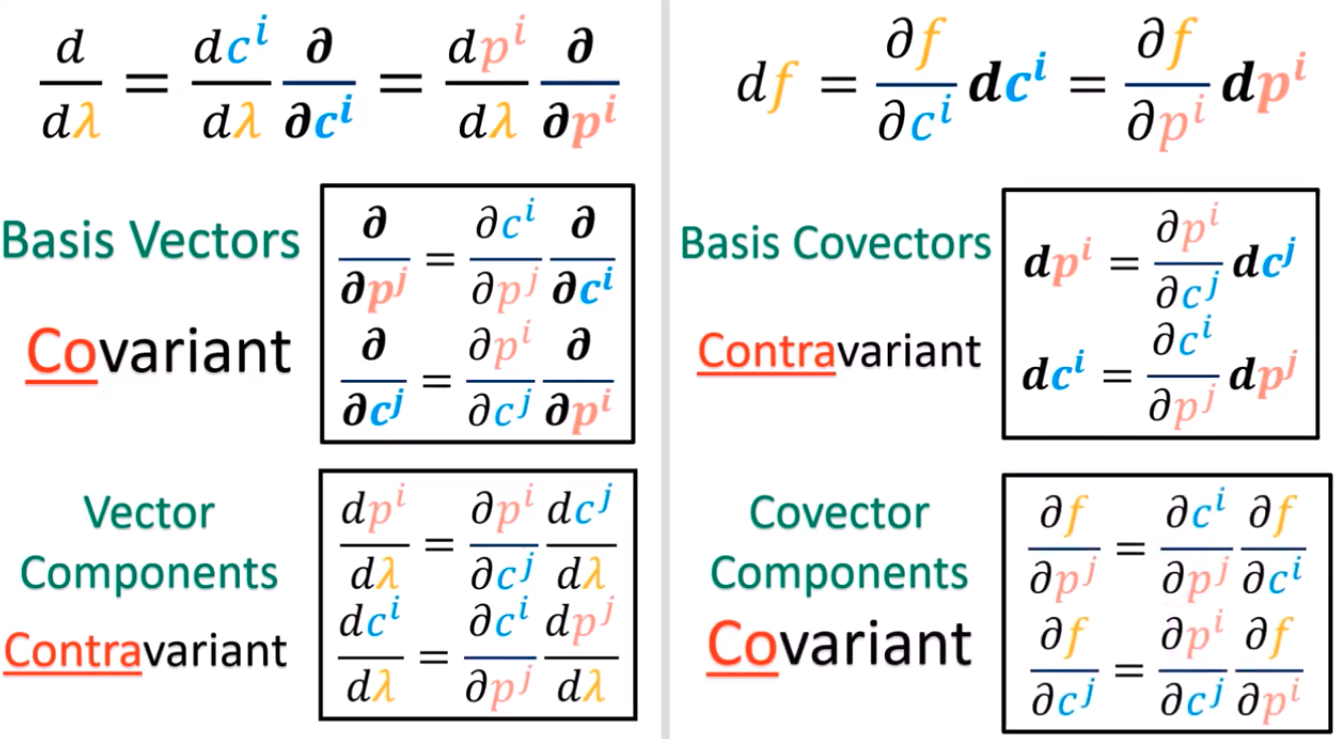
\includegraphics[scale=0.3]{figures/covector-field-xform-rules.png}
\end{center}